\section{Itération n°3}

\subsection{Objectif de l'itération}

Dans cette nouvelle itération, nous allons devoir modifier notre code afin que ce dernier puisse générer du bruit et gérer les problèmes au niveau du bruit et de sa puissance. Nous allons devoir coder une nouvelle classe afin qu'elle émette un bruit gaussien. Par ailleurs, nous devrons mettre en place un code nous permettant d'échantiller les signaux bruités reçu afin qu'ils correspondent aux signaux émis.

Ci-dessous le schéma correspondant à l'itération n°3.

\begin{figure}[h]
    \centering
    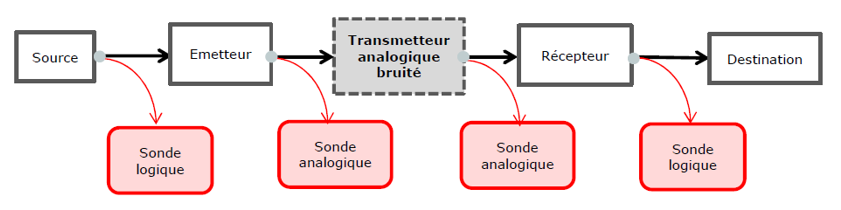
\includegraphics[width=1\textwidth]{image 16.png}
    \caption{\label{fig:image16}Schéma de l'itération n°3.}
\end{figure}

Ci-dessous le schéma correspondant à l'ajout de bruit pour cette itération

\begin{figure}[h]
    \centering
    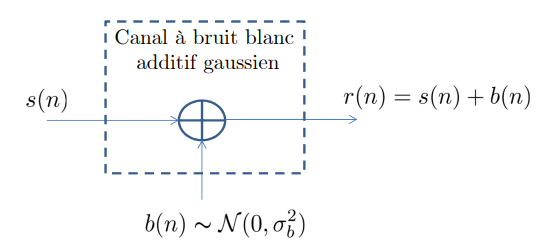
\includegraphics[width=0.8\textwidth]{image 17.png}
    \caption{\label{fig:image17}Schéma d'ajout de bruit itération n°3.}
\end{figure}

Dans cette partie on nous demande également un graphique représentant le taux d'erreur binaire (TEB) en fonction du rapport signal sur bruit (SNR) par bit. Nous devons donc faire des modifications dans notre code afin de calculer le SNR et de modéliser la courbe.

\subsection{Organisation}

Pour nous permettre de répondre aux demandes de l'itération (mise en place de l'ajout d'un bruit blanc gaussien), nous allons devoir créer de nouveaux éléments par rapport au code de l'itération précédente. Ces modifications devront nous aider à lancer le programme tout en prenant en compte le bruit qui pourrait se trouver dans un canal de transmission. Nous ne devrions pas avoir d'erreurs sur notre code cependant nous devrions pouvoir observer l'ajout de bruit que nous avons effectué sur nos graphiques lors de la modélisation de notre signal transmis à la destination. Afin de vérifier le bon fonctionnement de notre code nous nous appuirons sur ces graphiques mais également sur les calculs du TEB, du SNR ainsi que sur la courbe TEB vs SNR.
En vue des modifications à effectuer, nous avons développé le diagramme de Gant que nous avions utilisé lors de la première itération afin d'affecter à chacuns des tâches pour permettre de pouvoir livrer l'itération à l'heure. Vous trouverez ci-dessous le diagramme de Gant pour cette troisième itération :

\begin{figure}[h]
    \centering
    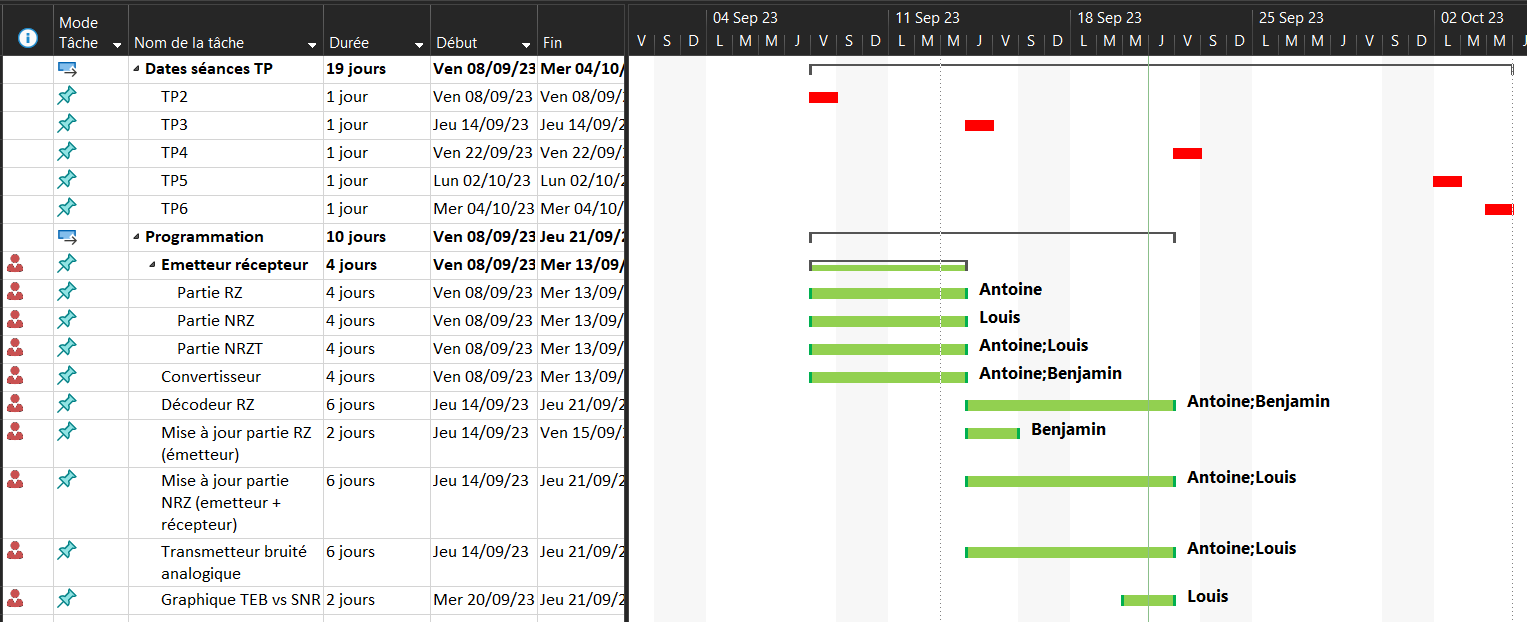
\includegraphics[width=1\textwidth]{image 18.png}
    \caption{\label{fig:image18}Diagramme de Gant itération 3 (1/2).}
\end{figure}
\begin{figure}[h]
    \centering
    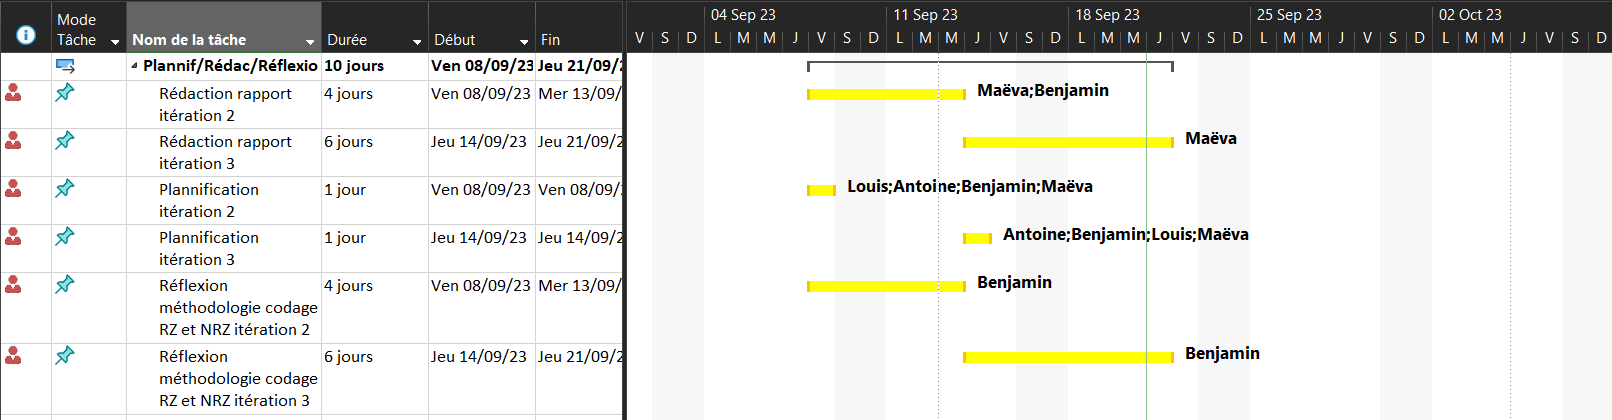
\includegraphics[width=1\textwidth]{image 19.png}
    \caption{\label{fig:image19}Diagramme de Gant itération 3 (2/2).}
\end{figure}

Pour le développement de notre code nous avons utilisé l'application de bureau Intellij Idea, comme évoqué pour la seconde itération. Nous utiliserons cette application tout au long du TP. Nous avons également utilisé GitLab nous permettant de stocker le projet. Nous l'utiliserons également tout du long du TP.

\subsection{Procédures de développement}

Afin de répondre aux exigences de l'itération nous avons créé une nouvelle classe de type de composant transmetteur qui se nomme TransmetteurBruiteAnalogique. Le transmetteur est un élément clé dans une chaîne de transmission. Dans notre cas, ce dernier est analogique et nous permet donc de transmettre un signal analogique à partir d'informations numériques faites à base de 0 et de 1.

Dans cette itération, nous nous intéressons à la modulation du bruit et de son ajout au code et au signal final. Afin de modéliser ce bruit nous avons besoin de formules mathématiques que nous pouvons retrouver par raisonnement.

\subsubsection{Modélisation du bruit}
Pour la création de notre bruit nous devons utiliser la méthode de Rice. Cette méthode est utilisée pour mesurer des longueurs d'arbre binaire en informatique et en théorie des graphes. Elle est utilisée pour modéliser la variation de l'intensité du signal lorsqu'il se propage à travers un canal de communication sans fil, en présence de diffusion multi-trajet (multipath fading). Par ailleurs, elle nous permet d'aider à modéliser le canal de transmission, étudier la performance du système et conceptualiser des systèmes de communication robustes. Elle sert à modéliser le fading multipath dans les canaux de communication et à évaluer l'impact de ce phénomène sur la performance des systèmes de communication.

\subsection{Tests}

\subsection{Performances}

\subsection{Conclusion}